\PassOptionsToPackage{quiet}{fontspec}
\documentclass{article}
\usepackage[UTF8]{ctex}
% Language setting
% Replace `english' with e.g. `spanish' to change the document language
\usepackage[english]{babel}

% Set page size and margins
% Replace `letterpaper' with`a4paper' for UK/EU standard size
\usepackage[letterpaper,top=2cm,bottom=2cm,left=3cm,right=3cm,marginparwidth=1.75cm]{geometry}

% Useful packages
\usepackage{amsmath}
\usepackage{graphicx}
\usepackage[colorlinks=true, allcolors=black]{hyperref}
\usepackage{amssymb}
\usepackage{titletoc}
\usepackage{titlesec}
\usepackage{fontspec}
\setmainfont{Times New Roman}
\usepackage{subfigure}
\usepackage{tikz}
\usetikzlibrary{positioning,petri}
\usetikzlibrary{arrows.meta,arrows,shapes,automata,backgrounds,petri,patterns,decorations.pathmorphing,positioning,calc,shapes.geometric}%插件
\usepackage{xcolor}
\usepackage{tcolorbox}
\usepackage{algorithmic}
\usepackage{diagbox}
\usepackage[ruled,vlined,linesnumbered]{algorithm2e}
\usepackage{tabu}
\usepackage{multirow}
\usepackage{booktabs}
\usepackage{framed}
\usepackage{hyperref}

\RequirePackage{xeCJK} 
\setCJKfamilyfont{KaiTi}{KaiTi} \newcommand{\song}{\CJKfamily{KaiTi}}


\hypersetup{
    colorlinks=true,
    linkcolor=black,
    filecolor=magenta,      
    urlcolor=blue,
    pdftitle={Overleaf Example},
    pdfpagemode=FullScreen,
    }







\titleformat{\section}{\normalfont\Large\bfseries}{\thesection.}{0.2em}{}
\titleformat{\subsection}{\normalfont\large\bfseries}{\thesubsection}{0.2em}{}

\newtheorem{definition}{Definition}
\newtheorem{example}{Example}
\newtheorem{problem}{Problem}
\newtheorem{remark}{Remark}
\newtheorem{derivation}{Derivation}
\newtheorem{proposition}{Proposition}




\begin{document}




\title{
\includegraphics[width=1.2in]{MUST.png}\\[-2pt]\huge Macau University of Science and Technology
	~\\
	Faculty of Innovation Engineering
	~\\
	Dept. of Engineering Science
	~\\
	\LARGE{(澳門科技大學創新工程學院工程科學系)}
	~\\[40pt]

	Thesis Proposal
	~\\
	(論文選題報告)
	~\\[40pt]

	\textbf{\LARGE Research on the Structure of Offline Handwritten Signature Verification Models Based on Transformer}

	\title{}

	~\\[50pt]





	\large{

		Submitted by: Mingchen Wang


		~\\[1pt]

		Student No.: 2230025907

		~\\[1pt]

		Supervisor: Xin Liu}

}

\author{}

\date{}


\titlecontents{section}[0pt]{\addvspace{5pt}\filright}
{\contentspush{\thecontentslabel\
	}}
{}{\titlerule*[8pt]{.}\contentspage}


\maketitle
\thispagestyle{empty}

\clearpage




\pagenumbering{roman}
\renewcommand{\abstractname}{\Large Abstract\\}
\begin{abstract}
	Offline handwritten signature verification is one of the application scenarios of biometrics technology, which is widely used in daily life for security authentication, financial transactions and other security fields based on the comparison between the handwritten signature provided by the user and the handwritten signature stored in the database to verify the user's identity. In academic research, offline handwritten signature verification consists of two types of tasks: Writer-Dependent and Writer-Independent. The first task is to verify the handwritten signature against the handwritten signature of the corresponding user in the database. The second task is to determine whether the handwritten signature is forged or not only by the provided handwritten signature. In the experimental part of this paper, it conducts comparison experiments based on the above tasks to verify the accuracy of the proposed deep learning model structure.

	The research content of this paper is as follows: 1. Recover relevant offline handwritten signatures to verify the deep learning model structure, and analyze the defects of the model in each stage. 2. proposing a CNN+Transformer end-to-end multi-scale feature extraction model OSVTF for offline handwritten signature verification, which can solve some of the shortcomings of CNN or Transformer in image feature learning, and the combination of these two can have better image feature learning ability. 3. In the classifier part, support vector machine and global average pooling + classification head are used to select a better classifier according to the experimental results.

	Based on the above research, a feature extractor with both CNN and Transformer image feature learning capability is proposed to provide a CNN+Transformer style model structure idea for the derivation of image classification task. In daily life, it can help security personnel to better verify whether a handwritten signature is the work of the person, and thus better protect personal privacy and property security.

	\textbf{keywords}: Offline handwritten signature verification; end-to-end; CNN; Transformer; OSVTF.
\end{abstract}

\phantomsection\addcontentsline{toc}{section}{Abstract}\tolerance=500



\newpage


\clearpage

\renewcommand{\abstractname}{\Large 摘要\\}
\begin{abstract}
	\medskip
	離線手寫簽名驗證是生物特徵技術的一個應用场景, 其根據用戶提供的手寫簽名与資料庫中該用戶存儲的手寫簽名進行對比以驗證用戶身份, 在日常生活中被廣泛用於安全認證, 金融交易等安全領域. 學術研究中, 離線手寫簽名驗證包含兩種類型的任務: 作者依賴和作者獨立. 第一種任務是將手寫簽名與資料庫的對應用戶手寫簽名進行對比驗證. 第二種任務是僅通過提供的手寫簽名來判斷是否偽造的. 本文在實驗部分會根據上述任務進行對比實驗, 以驗證提出的深度學習模型結構準確率.

	本文研究内容如下: 1. 復現相關的離線手寫簽名驗證深度學習模型結構, 分析各個階段的模型存在的缺陷. 2. 提出CNN+Transformer的端到端多尺度特徵的離綫手寫簽名驗證特徵提取模型結構OSVTF, 解決CNN或Transformer在圖像特徵學習的部分缺陷, 並且這兩者相加的組合方式能夠擁有更優秀的圖像特徵學習能力. 3. 在分類器部分, 使用支持向量機、全局平均池化+分類頭兩種方法, 根據實驗結果選擇更優秀的分類器。

	基於上述研究, 提出一個同時擁有CNN和Transformer圖像特徵學習能力的特徵提取器, 為圖像分類任務的衍生分支提供一個CNN+Transformer風格的模型結構思路. 在日常生活中能夠幫助安全領域人員更好地驗證手寫簽名是否為本人的工作, 從而更好保護個人隱私和財產安全.

	\medskip
	\textbf{關鍵詞}:離線手寫簽名驗證; 端到端; CNN; Transformer; OSVTF.
\end{abstract}

\phantomsection\addcontentsline{toc}{section}{摘要}\tolerance=500

\newpage



\ctexset{ contentsname = {Table of Contents}}

\tableofcontents

\phantomsection\addcontentsline{toc}{section}{Table of Contents}\tolerance=500
\newpage

\pagenumbering{arabic}
\setcounter{page}{1}

\section{Introduction}
\subsection{Research Background}

Biometrics technology is a technology for identification or verification based on individual physiological features such as fingerprints, face, iris, or behavioral features such as voiceprints and handwritten signatures. This technology is widely used in security fields such as security authentication in enterprises, financial transactions, access control systems, etc \cite{1}.

The technology is mainly used in recognition and verification scenarios. In the first scenario, the user only needs to provide samples of individual or physiological features, and the biometric system recognizes the user who provides the features among the registered users based on the samples. In the second scenario, on the other hand, based on the first scenario, the user declares his/her identity to the system, and then the system will verify whether the specified user is one of the registered users based on the above information.

Handwritten signature is a more important individual behavioral feature in daily life because it serves as the main feature for verifying personal identity in legal, financial, and administrative fields. Also, because it cannot be invaded during the collection process, handwritten signatures are considered as one of the main features in many technologies for verifying personal identity. This gives rise to the specific application of handwritten signature verification, based on the user-provided signature (defined as Query) and the user's stored signature (defined as Reference) in the system for comparison and verification, so as to identify the identity of the statement is true.
Handwritten signatures are categorized into two types, offline and online, depending on the collection route. The collection process of offline handwritten signatures is obtained by the user after the writing process on the paper; online handwritten signatures are collected using a digitizing station, and the collected handwritten signature images may be affected by the equipment, such as the position of the pen, tilt, pressure, etc. \cite{3}. Therefore, offline handwritten signature has the advantage of collecting user's personal signature image anytime and anywhere without the limitation of devices, and people prefer to write their personal signatures on paper.

With the development of the level of technology, the field of artificial intelligence has been able to provide the user with a few sample graph images and a few keywords, so as to generate a fake image, and normal people are difficult to identify the true and false naked eye. Therefore, there will be some people to generate forged signatures, so as to achieve the fake to pass the verification of the security system, resulting in the invasion of personal privacy, personal property theft and other dangerous consequences. In daily life and work, many scenes need to use to offline handwritten signature verification, rely solely on manual power to verify there will be a certain degree of social risk and judgment errors, so the study of offline handwritten signature verification, to a certain extent, can reduce the risk of forged signatures through the verification system, to a certain extent, reduce the error of manual verification, so as to ensure the individual's right to privacy and property security.

\newpage

\subsection{Motivation}

Offline handwritten signature verification is essentially an image classification task, where the input is a signature provided by the user and the signature of that user that already exists in the repository, thus comparing these two image features and finally outputting whether this signature is a forgery or not. Unlike traditional image classification tasks, the input is not a single color or gray image, making this task a newer challenge. Studying this direction can to some extent learn the direction of derivation of the input pair of features branch of the image classification task, and provide a kind of basic idea or model for the subsequent image classification task that requires the input to be a pair of features.

Although handwritten signatures in the collection process will not be affected by the digitizing table and other equipment factors, but the user uses paper to write personal signatures can not guarantee that the signature obtained from multiple writings is exactly the same, and may also be affected by the physical pen, paper thickness and so on. Therefore, the data pre-processing process to a certain extent will directly affect the system verification effect, and a pair of pictures of the data pre-processing whether to take the same processing method is also worth studying, a pair of pictures of different data pre-processing methods will improve the final verification effect.

In the past research on offline handwritten signature verification, scholars design image feature extraction methods based on data cluster characteristics such as sample distribution, and adopt traditional machine learning methods to verify whether the signature is forged \cite{1}. However, this method has defects, the verification credibility and accuracy rely heavily on manually designed features, and there are restrictions on the font style of handwritten signatures, etc., and the time cost of data preprocessing is very huge. With the development of deep learning, in recent years, scholars have gradually adopted deep learning methods such as convolutional neural networks (CNN) for offline handwritten signature verification, in which the model architecture obtained by supervised learning through model parameter training has been experimentally shown to achieve better results in offline handwritten signature verification \cite{2}. Therefore, the deep learning model architecture greatly and directly affects the accuracy of offline handwritten signature verification, and a single deep CNN or Transformer \cite{9} model architecture for offline handwritten signatures in recent years will be missing some key image features to a certain extent, while CNN's excellent image local feature learning ability and Transformer's excellent global feature learning ability just complement each other. Global feature learning capability of CNN just complement each other, so the proposed CNN+Transformer style model architecture for offline handwritten signature verification in this paper may outperform the current CNN or Transformer model architecture in terms of accuracy.

\newpage

\subsection{Research Objectives}

Offline handwritten signature verification consists of two tasks: Writer-Dependent (WD) and Writer-Independent (WI). the WD task requires Reference and Query to verify the handwritten signature samples to verify whether the signature is forged or not, and to a certain extent, it will rely on the characteristics of the Reference of the writer. the WI task is to verify whether the signature is forged or not by Query only. The WI task is to verify whether the signature is forged or not by using Query only, and does not depend on the Reference feature of the writer.

For the WD and WI tasks, the main objectives of this paper are as follows: 1. Reproducing OSV (Offline Signature Verification) Deep Learning Models; 2. Propose a CNN+Transformer style OSV model architecture to extract one-to-one handwritten feature image features to address some of the shortcomings of CNN or Transformer understanding of image features; 3. Propose classifiers that better fit the above OSV model and can better utilize the image features extracted by CNN+Transformer.

In the first phase, the existing newer OSV models are reproduced to analyze and summarize the OSV model architectural details and features, and to find out the commonalities and shortcomings among them, so as to better find the optimization key points and methods.

In the second phase, a CNN+Transformer style OSV model architecture is proposed on the basis of the reproduction model. Multi-scale features of CNN are added to the Encoder-Decoder architecture of Transformer, thus enhancing the model to learn image features at each scale. Model training will take place in comparative experiments to verify the model credibility and quality. During the comparison experiments, the image preprocessing and validation methods are constrained to be consistent, so as to find out the final training and validation scheme suitable for the model architecture.

In the third stage, since the convolutional neural network in the image classification task is different from that of the offline handwritten signature verification task in terms of the final output category probability, the previous offline handwritten signature verification algorithms or models have taken the support vector machine to identify whether the signature is a forgery or not. In the proposed CNN+Transformer style OSV model as a feature extractor, there is some difference from the feature extraction part of traditional machine learning for offline handwritten signature verification. As a result, in the probability stage of whether the output after feature extraction is a forgery or not, whether adopting the global average pooling and fully connected layer of CNN in the image classification task has better performance than the traditional machine learning support vector machine needs to be experimentally verified for the WI and WD tasks.

\newpage
\section{Literature Review}

The image data collected by offline handwritten signature for model or algorithm validation needs to undergo certain preprocessing, and good data preprocessing techniques will improve the system validation accuracy to a certain extent. In order to improve the quality of signature images, scholars have taken the processing of RGB image conversion to GRAY single-channel image, and some even use the image processing of smoothing pixels in order to remove the noise \cite{4}. This processing method can well reduce the unnecessary features of handwritten signature images collected on white paper, such as RGB three-channel image in some channels of the pixel points of the value of 255, while the pixel points with handwriting handwriting tend to be very small in value. However, this processing method has the defect that the value of the pixel points in the part with handwriting features is very small, while the value of the pixel points in the other blank parts is very large, so subsequent scholars have processed these images with black and white inversion, and it has been verified that this processing method can obtain a better verification accuracy \cite{4}.

The early days of offline handwritten signatures were all machine learning approaches, e.g., Edson et al. proposed an offline signature verification system using Hidden Markov Models \cite{5}. This traditional machine learning approach is flawed: it relies on manually designed features for training, and the accuracy of classification is directly related to these features \cite{2}. Therefore no matter how much the model is replaced in the classification stage, it still takes a lot of time to extract signature image features in the data preprocessing and feature extraction stage. In 2005, Edson et al. conducted comparative experiments on SVM and HMM for offline handwritten signature verification \cite{6}, and the experimental results showed that SVM was better than the statistical model of HMM.SVM is a widely-used machine learning technique, which is favored because of its high efficiency in binary classification tasks \cite{7}, and offline signature verification is essentially a binary classification task that belongs to the category of identifying whether signatures are forgeries or not, so the subsequent offline signature verification is a binary classification task that belongs to the category of identifying whether signatures are forgeries or not. binary classification task, so most of the subsequent offline handwritten signature verification tasks on take SVM as a classifier, more focused on image preprocessing and extracting handwritten signature image features.

With the development of deep learning and convolutional neural networks, in 2012 Krizhevsky A. et al. proposed AlexNet \cite{8} to win the image classification task of the ImageNet competition far ahead of the second participant using traditional algorithms, which made the deep learning represented by convolutional neural networks gradually become the mainstream method of the image task task. Subsequently, academics introduced a deeper convolutional neural network VGG \cite{9}, which is an architecture that adds more convolutional layers on top of AlexNet to extract more channels of feature maps. But this way of stacking convolutional layers will lead to the size of the extracted feature maps become smaller at the same time, leading to the loss of features of other sizes, in order to solve this problem, in 2016 He Kaiming et al. proposed ResNet with residual connectivity \cite{10}.These convolutional neural networks, ResNet and VGG, are similar in that they are superimposed with a number of convolutional layers, but in each size of the feature map, a residual connection is added between the convolutional layers. The feature maps of the original input convolutional layers are accumulated onto the feature maps of the output of the convolutional layers, thus preserving some of the original features of that size. This approach in supervised learning convolutional neural networks, after weight sharing convolutional kernel operations, can somewhat compensate for the original image feature information, and this residual connection approach has become a mainstream approach for subsequent neural network models. The quality performance of convolutional neural networks on image classification tasks has led to other domains to borrow this convolutional neural network approach in order to accomplish tasks, and the same is true for offline handwritten signature verification. In 2017, L. G. Hafemann et al. used a convolutional neural network for offline handwritten signature verification \cite{11}, which is the same as the CNN for image classification tasks, and both take a convolutional layer + max pooling layer to extract the handwritten signature image feature maps, with a slight difference in the final output portion; the model is to take the features of the final fully-connected layer and pass them through two output The model has two outputs: author prediction and forgery prediction. The model requires the input to be a single handwritten signature image instead of adult handwritten signature images, which belongs to the WI task, while the WD task requires Reference.The paper provides a supervised learning approach for handwritten signature image feature extraction, and the experimental results prove that this approach significantly improves the accuracy of offline signature verification, laying a foundation for the subsequent handwritten signature verification using CNNs and deep neural networks. Laying the foundation for subsequent handwritten signature verification using CNNs and deep neural networks.

The above mentioned convolutional neural network uses a convolutional kernel to traverse image pixels to learn image features, but the convolutional operation has the defect of local field of view. Although it can learn local features of an image, it is less effective in learning global features, so scholars have successively proposed ResNet's residual connectivity and FPN-Style \cite{12}, a multiscale network for target detection, to optimize these problems, but it does not address the root cause of the lack of global feature capability and the image is bound to be accompanied by redundant information and useless pixel points. With the development of the field of natural language processing with deep learning, in 2017 Vaswani A. et al. proposed the Transformer model for machine translation \cite{13}. The model adopts the Encoder-Decoder mainstream architecture for machine translation, and unlike previous deep learning models for machine translation, Transformer introduces an attention mechanism. Under the action of the attention mechanism, it is able to perform global feature perception on word vectors, and refer to the feature information of the previous word and the feature information of the input word vectors when generating the predicted words, so it can generate sentence predictions of different lengths. And the experiment proves that Transformer has better global generalization ability than the previous Encoder-Decoder machine translation model.

In view of the Transformer's ability to perceive global features with attention, Dosovitskiy A. et al. first used the Transformer Encoder for image classification task in 2021, named Vision Transformer (ViT) \cite{14}. The internal structure of ViT completely abandons the convolutional layer, and takes the input image as a word vector after patch and Embeddings operations. The internal structure of ViT completely abandons the convolutional layer and takes the input image as a patch and Embeddings operation, the embedding of each patch is treated as a single token of word vectors, and then the image is flattened and entered into the Transformer Encoder as word vectors, which is passed through a number of Encoder Layers, and then a MLP is set up to map category probabilities in order to complete the image classification task. The task of image categorization is accomplished. Experiments have shown that this way of modeling has obtained recognition accuracy ahead of convolutional neural networks on image classification tasks, from which deep learning model architectures of CNN + Transformer have also been derived, such as DETR for image target detection \cite{15} and MaskFormer for image segmentation \cite{16}. This approach takes a Linear layer convolutional neural network that removes the final classification, inputs the image to extract multi-channel features, and uses the features as input vectors to the Transformer to perform global feature sensing.DETR, the pioneering work of CNN + Transformer, is validated in MS COCO \cite{17}, although the validation effect is not as good as the previous R-CNN \cite{17}, which adopts the post-processing operations such as NMS. R-CNN \cite{18}, YOLO series network \cite{19}, the recognition accuracy is high, but the advantage of this approach is that it does not need any pre-setting of target detection a priori box such as Archer Box and NMS post-processing, which is an end-to-end model architecture. This approach simplifies the model inference process to a certain extent, but it also increases the cost of model training time, and requires the design of a finer training scheme to ensure the convergence of model parameters.

Transformer has excellent global feature perception capability compared to CNN on image tasks, so scholars in the field of offline handwritten signature verification have proposed a Transformer-based model architecture TransOSV \cite{20}. The model adopts similar Encoder-Decoder architecture, the input Reference and Query are pre-processed by RGB to GRAY image, and then enter into the ViT Encoder as Holistic Encoder, then the output of Holistic Encoder is subjected to convolution operation, and finally the features of Reference and Query are subjected to Contrastive Encoder. and Query features for Contrast based Part Decoder operation. In the training process, TransOSV aggregates the output class features of Transformer Encoder, the output features of Convolution Module and the output features of Decoder to compute the training loss to complete the model training, and finally the feature classifiers also adopt the Support Vector Machines to verify whether the signature is forged or not. The architecture in Decoder's Cross-attention will Reference features and Query features for attention calculation, the Reference and Query features for the relevance of attention learning, can be better linked to the relationship between Reference and Query. But this architecture will lack the image multi-channel feature information to some extent because the input image is directly patched and Embeddings into the Transformer Encoder. Since the image size of ViT is globally constrained, some key information will be lost when the image is resized.

In summary, based on the TransOSV architecture, this paper will take the CNN + Transformer approach, add a new backbone to extract the multi-channel feature map by CNN before the image enters the Transformer Encoder, and then extract the multi-scale feature map of the backbone for flattening and splicing to supplement the handwritten signature image features before entering the Transformer Encoder. The subsequent decoding part introduces the multi-scale feature map features to form the Transformer offline handwritten signature verification feature extraction model that is adapted to multi-scale handwritten signature image features. After the feature extraction the classifier will take the global average pooling and classification header in order to verify whether the handwritten signature is a forgery or not.

\newpage
\section{Offline Signature Verification TransFormer}

\begin{figure}[htbp]
	\centering
	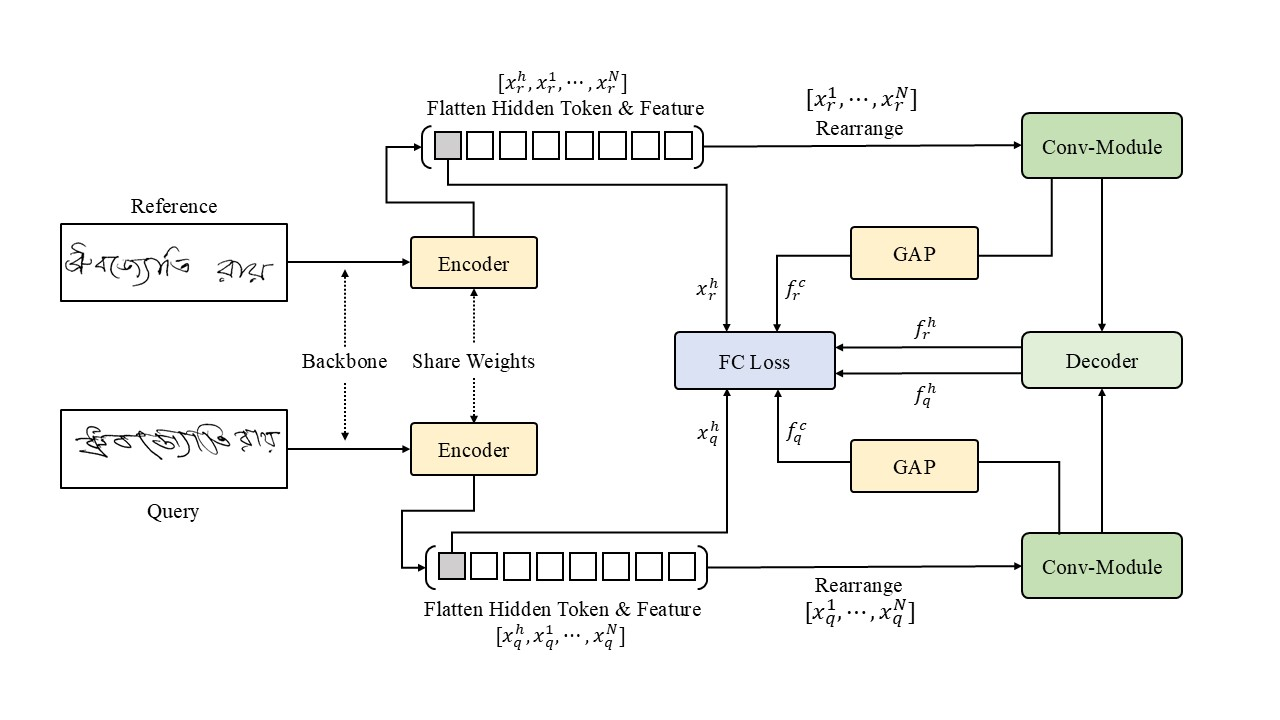
\includegraphics[scale=0.5]{figure/p1.jpg}
	\caption{Offline Signature Verification TransFormer (OSVTF)}\label{fig:p1}
\end{figure}

\subsection{Overview}

The proposed OSVTF is shown in Fig. 1. Input a pair of handwritten signature images with the same size Reference (R) and Query (Q), firstly extract the multi-scale feature map through Backbone, and then the multi-scale feature map will be flattened and spliced through the weight-sharing Encoder in order to learn the image features, and this part of the inference will be extracted to obtain a pair of flattened feature token $x_r^e,x_q^e$ and a pair of flat feature map $[x_r^1,\cdots,x_r^N],[x_q^1,\cdots,x_q^N]$. Subsequently the flat feature map will go through reshape to 2D image vectors before inference by convolution module. The output of the convolution module will be divided into two directions: the first direction will pass through the Global Average Pooling layer to get the flat convolutional features $f_r^c,f_q^c$; and the other direction will pair into the Decoder to get the flat attentional decoding features $f_r^d,f_q^d$. The training process will collect the flat feature tokens $x_r^d,x_q^d$ in the inference process, and the training process will collect the flat feature tokens $x_r^h,x_q^h$ in the inference process. $x_r^h,x_q^h$, flat convolutional features $f_r^c ,f_q^c$ and flat attentional decoding features $f_r^d,f_q^d$ during the inference process will be collected to perform Focal Contrast Loss (FC) loss computation to train the model weights. The Encoder, Decoder and Conv-Module structures are analyzed in depth next.

\subsection{Backbone}

\begin{figure}[htbp]
	\centering
	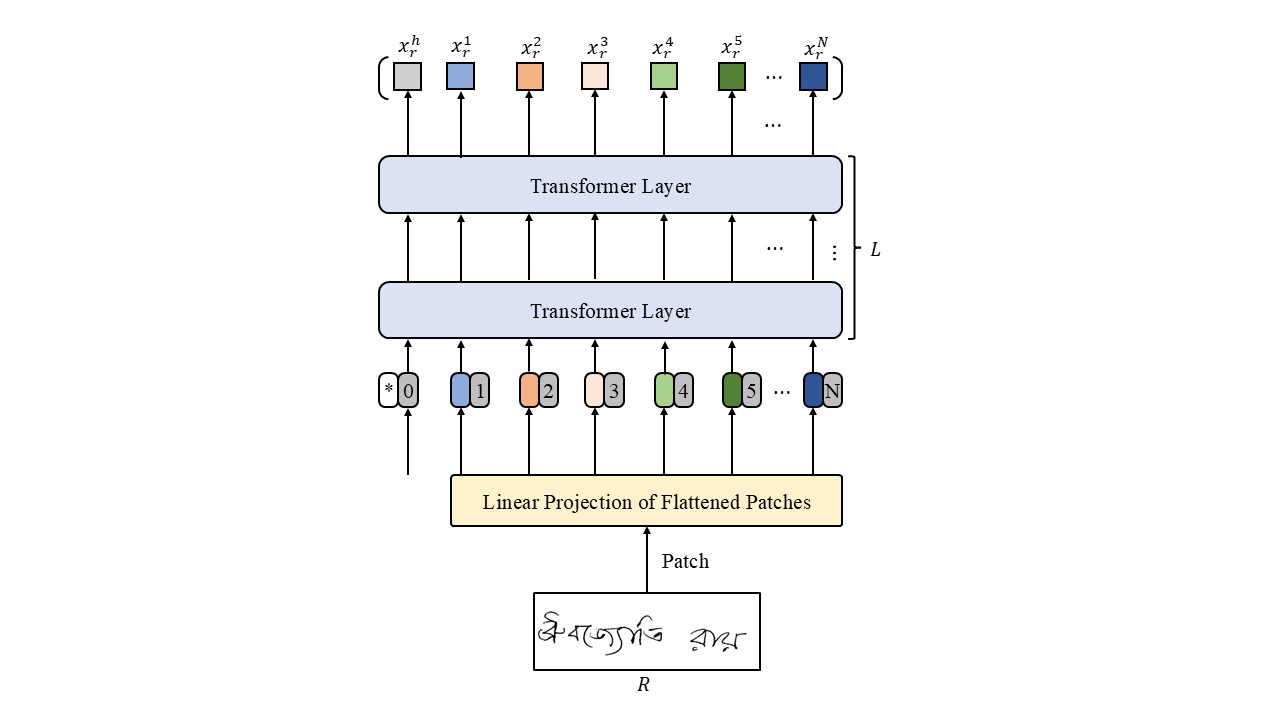
\includegraphics[scale=0.5]{figure/p2.jpg}
	\caption{Backbone structure}\label{fig:p2}
\end{figure}

Taking the architecture of CNN on Backbone, the image is fed into a convolutional neural network, and a multi-channel feature map will be obtained after the operation of the convolutional layer. As shown in Fig. 2, taking ResNet-50 as an example, the input reference signature image $R \in \mathbb{R}^{H\times W\times C}$, where H, W, and C denote the height, width, and number of image channels. First R passes through the first convolutional layer and the output feature map of Conv1 is calculated per pixel point as follows in eq.\ref{eq:e1}.

\begin{equation}\label{eq:e1}
x_r^{b_1}[i,j,k] = \sum_{m=0}^{H_{k1}-1} \sum_{n=0}^{W_{k1}-1} \sum_{c=0}^{C-1} R[i+m,j+n,c] \cdot W_1 [m,n,c,k] + b_1[k]
\end{equation}

where $x_r^{b_1}[i,j,k]$ denotes the value of the output feature map of the first block (Conv1) in the backbone on the kth channel at position $(i, j)$; $W_1,b_1$ denote the convolution kernel weights and bias of Conv1; $H_k,W_k$ denote the height and width of the convolution kernel; and m,n denote the convolution kernel position index. Each of the subsequent Conv2D operations in Conv2, Conv3, Conv4, and Conv5 are the same as above.

ResNet-50 is different from traditional CNNs in that after a certain number of convolutional layer operations, such as the Conv2 part of Fig. 2, a residual join is performed, i.e., the feature maps prior to the input of the current convolutional layer are accumulated to the feature maps after the current convolutional layer operation, so as to make up for some of the missing features in some of the convolutional operations. The reference signature image features for each block are computed as follows in eq.\ref{eq:e2}.

\begin{equation}\label{eq:e2}
x_r^{b_{l+1}} = f(x_r^{b_l}, W_l) + x_r^l
\end{equation}

Where $l$ denotes the lth block in the backbone, e.g., $l=1$ denotes Conv1; $f(x_r^{b_l}, W_l)$ denotes one or more convolution operations that the feature image $x_r^{b_l}$ undergoes, e.g., when $l=2$, $x_r^{b_2}$ will undergo 3 times of the layers stacked by 3 convolution operations. After one stacked convolution operation, in order to solve the problem of difficult convergence of training, the Rectified Linear Unit (ReLU) \cite{21} activation function and Batch Normalization (BN) \cite{22} operation are used.The idea of the ReLu activation function is that when $x>0$, the ReLU output is linear; on the contrary, when $x\leq 0$ ReLU output is 0. The formula is as follows in eq.\ref{eq:e3}.

\begin{equation}\label{eq:e3}
f(x) = \max(0,x)
\end{equation}

The idea of BN is to normalize the current batch mean μ and variance $\sigma^2$ of the current operation output during the model batch training, while the global mean and variance accumulated during training are used in the inference phase. The computational formula is as follows in eq.\ref{eq:e4}

\begin{equation}\label{eq:e4}
\hat{x}_{i,j}= \frac{x_{i,j} - \mu_j}{\sqrt{\sigma_j^2+\epsilon}}
\end{equation}

Under the current formula, $x_{i,j}$ denotes the value of the ith sample at the $j$-th feature.

In the OSVTF proposed in this paper, unlike the way of DETR, after the backbone operation, all the output feature maps of $l=2,3,4,5$ are all stitched together and then fed into the Encoder for subsequent operations as a way of increasing the multi-scale signature image features.

\subsection{Encoder}

Encoder is following the model structure of ViT (Vision Transformer) \cite{14} shown in Fig. \ref{fig:p3}.

\begin{figure}[htbp]
	\centering
	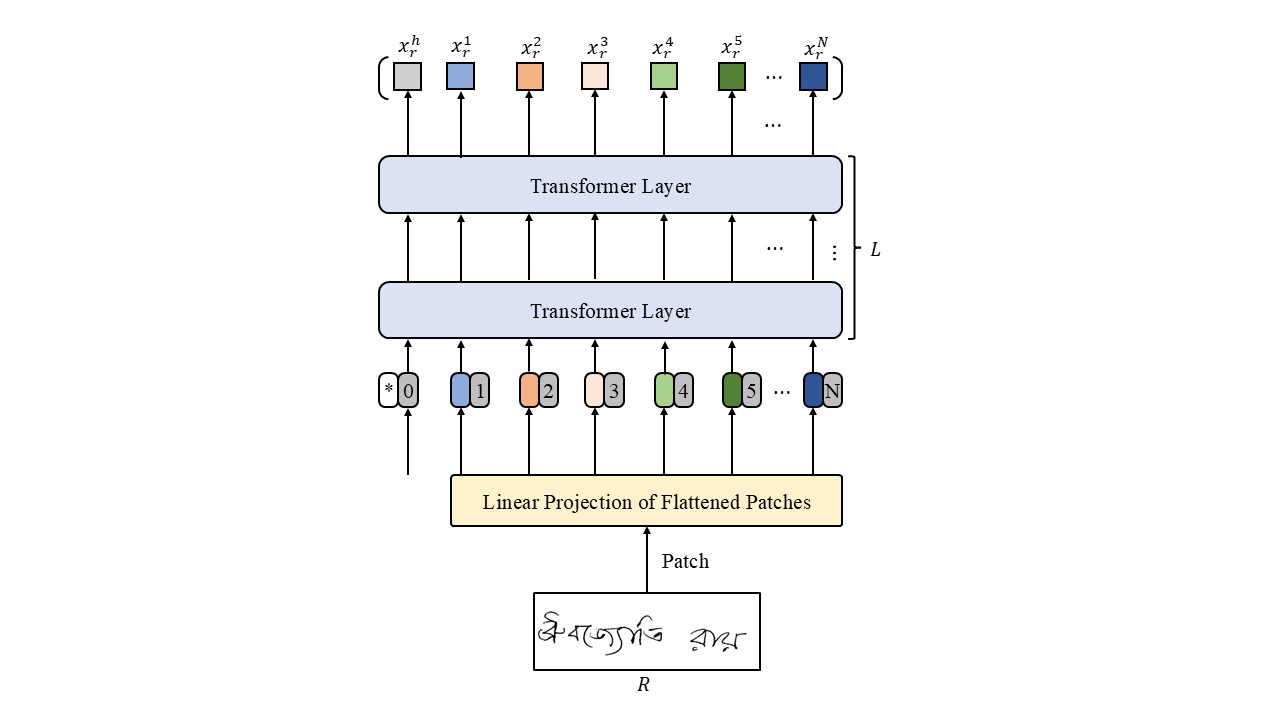
\includegraphics[scale=0.45]{figure/p3.jpg}
	\caption{Vision Transformer structure}\label{fig:p3}
\end{figure}

ViT first divides the input feature map into N blocks and flattening, where the patch number is calculated as in the following eq.\ref{eq:e5}.

\begin{equation}\label{eq:e5}
	N = [\frac{(H-P+S)}{S}]*[\frac{(W-P+S)}{S}]
\end{equation}

where $[\cdot]$ denotes the floor function. p and S denote the patch size and the number of convolutional layer steps, respectively, since the original ViT structure takes a convolutional layer in order to accomplish the chunking operation. Next, a learnable weight Class Token and patch image accumulation Position Embedding are spliced in the shape of $(N+1)\times(H\times W)$. Since the Transformer Encoder requires the input to be a Token vector, the relative position information will be lost after the image is patched, so the accumulated Position Embedding reassigns the relative position feature. After the above processing into the L layer Transformer Encoder Layer inference to get the Encoder's flat feature token with feature map $[x_r^h,x_r^1,\cdots,x_r^N ]$,$[x_r^h,x_q^1 ,\cdots,x_q^N]$, the whole Encoder inference as in equation (\ref{eq:e6}).

\begin{equation}\label{eq:e6}
	x_r=[x_r^h,x_r^1,\cdots,x_r^N ]=\mbox{Encoder}([\overline{x}_r^h,E(\overline{x}_r^1),\cdots,E(\overline{x}_r^N )]+pos)
\end{equation}

Where $E(\cdot)$ denotes Embeddings. pos denotes Position Embeddings. each Encoder has the same structure and is formed by $L$ stacks, as shown in Fig. \ref{fig:p4}.

\begin{figure}[htbp]
	\centering
	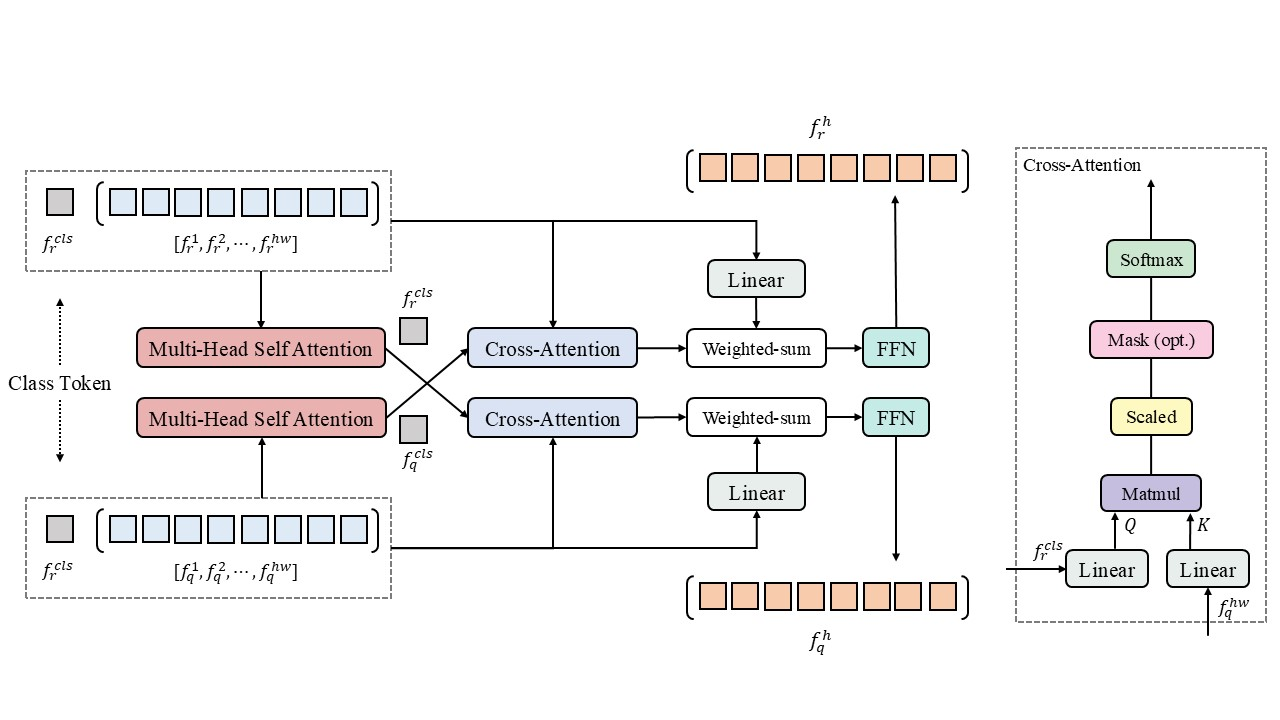
\includegraphics[scale=0.45]{figure/p4.jpg}
	\caption{Multi-Head Attention and Scaled DotProduct Attention}\label{fig:p4}
\end{figure}

Each Encoder Layer consists of a Multi-Head Self Attention (MHSA), Feed Forward Network (FFN), and two Residual Accumulation \& Layer Normalization (LN). First of all, before the input Token enters the Encoder, it will go through three Linear layers to map the input vectors to get $Q,K,V$, and input the mapped three vectors into the MHSA for the attention feature computation. The MHSA in Encoder is taken to be the same as the MHSA in Transformer \cite{13}, both of which use Scaled Dot Product Attention, which is calculated as in Equation \ref{eq:e7}.

\begin{equation}\label{eq:e7}
	\mbox{Attn}(Q,K,V)=\mbox{Softmax}(\frac{Q^T K}{\sqrt{d_k }})\cdot V
\end{equation}


where $d_k$ denotes the number of $K,V$ dimensions of the MHSA. Since Scaled Dot Production Attention involves two matrix multiplications of larger size in the computation process, the input process is based on the number of defined heads in order to generate the $d_k$ dimensional linear mapping weights of the number of heads multiplied by 3, which is used to map the input vector into the lower dimensionality of the three matrices $Q,K,V$. At each head, $Attn(Q,K,V ) $operation is performed on each head, and the resulting matrices from the attention computation are finally mapped to the input vector dimensions by a large linear layer. The resulting stacked Transformer Encoder is able to perform the MHSA computation multiple times to better learn the overall vector features.

\subsection{Conv-Module}

The input images are all flattened feature vectors after Encoder, so they need to be reshape to be able to carry out the convolution operation. At the same time, some 2D information will be lost after flattening Token, so the convolution module can make up for some 2D information after reshape. The composition of the convolution module is similar to that of the convolutional neural network, which consists of four Conv2D+ReLUs and two Max Pooling 2Ds in the order shown in Table \ref{tab:t1}.

\begin{table}[htbp]
	\caption{Conv-Module structure information}
	\begin{center}
		\begin{tabu} to 0.8\textwidth{X[2,c]|X[2,c]|X[2,c]}
			%0.8\textwidth   为设置表格宽度  
			%X[c]      表示这一列居中,所占比例为1,相当于X[1,c]  
			%X[3,c]   表示这一列居中,所占比例为3,这列的宽度是X[c]列的3倍  
			\hline
			Layer          & Kernel Size & Output shape              \\
			\hline
			Conv 2D + ReLU & $3\times 3$ & $d_c\times h\times w$     \\
			Conv 2D + ReLU & $3\times 3$ & $d_c\times h\times w$     \\
			Max Pooling 2D & $3\times 3$ & $d_c\times h/2\times w/2$ \\
			Conv 2D + ReLU & $3\times 3$ & $c\times h/2\times w/2$   \\
			Conv 2D + ReLU & $3\times 3$ & $c\times h/2\times w/2$   \\
			Max Pooling 2D & $3\times 3$ & $c\times h/4\times w/4$   \\
			\hline
		\end{tabu}
	\end{center}
	\label{tab:t1}
\end{table}

The output obtained after Conv-Module is propagated in two directions: the first direction is to perform Global Average Pooling (GAP) computation and flattening to obtain the flat convolutional features $f_r^c,f_q^c$; the other direction is to enter the Decoder in pairs for decoding attention computation.

\subsection{Decoder}

\begin{figure}[htbp]
	\centering
	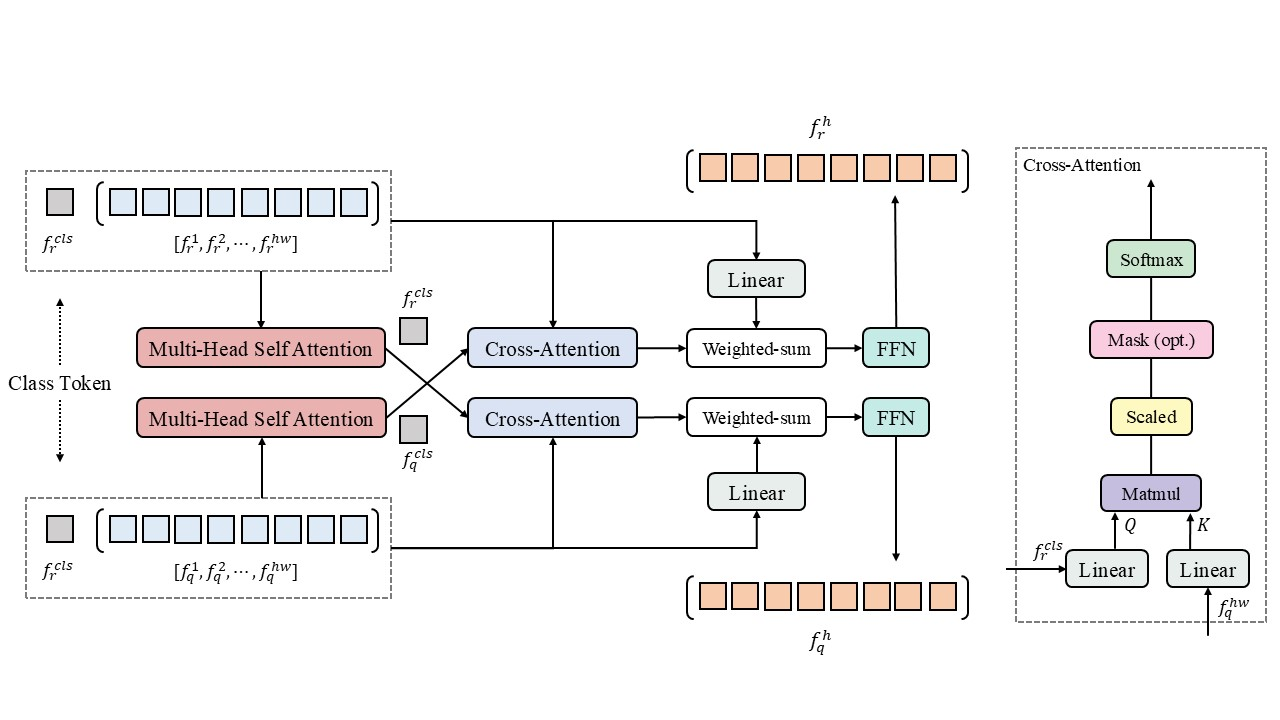
\includegraphics[scale=0.45]{figure/p5.jpg}
	\caption{Decoder and Cross-Attention}\label{fig:p5}
\end{figure}

The Decoder in OSVTF is different from the Transformer Decoder in that it takes two MHSAs and Cross-attention as shown in Figure 4-(a). Similar to the ViT input stage, before inputting the flattened convolutional features, a pair of learnable parameters with the same number of dimensions as the flattened convolutional features, defined as Class Token, is initialized.Its role is the same as that of the Class Token of the ViT-Encoder, which both define an adjusted weight for it to learn whether an image is a forgery or not in a new dimension, thus enabling the model to learn image features better.

Like the above MHSA, the formula is as in Eq. (\ref{eq:e7}).The flat convolutional features inserted with the class token are firstly subjected to MHSA in the Decoder to obtain the flat feature vector of the attention mechanism. Subsequently, in order to be able to learn the relationship between reference and query, Cross-attention is introduced as in Fig. 4-b. Based on the attention mechanism, the linear mapping of $f_r^{cls},f_q^{cls}$ is defined as the Query matrix, and the flattened attention features of the MHSA output are the Key matrix. Similar to MHSA, the attention mechanism is computed based on the learnable parameter class token of reference or query, and in addition the flattened features of the images, to some extent the query matrix inside the attention mechanism can reflect the attention between the images, and since there is no input value Value matrix, Cross-attention gets the attention weights $M_r ,M_q$. This mask weight contains the attention weights of each Token (i.e., each pixel point) between the reference and query, and thus the features of the input Decoder are then accumulated with the attention weights after broadcasting with the Embeddings, and thus what is obtained is a pair of flattened attention features of the attention mechanism. The final Decoder output $f_r^d,f_q^d$ is obtained after FFN, and this pair of features will be subsequently used to optimize the Decoder model parameters according to FC Loss.

\subsection{Loss Function}

The training process of OSVTF will take two loss functions; Sparsity Loss, Focal Contrast Loss.

\subsubsection*{Sparsity Loss}
Since only a few regions in the image of OSV contain discriminative information for signature verification task and $M_r,M_q$ in Decoder has sparsity, the calculation of cross entropy will be taken in order to generate a diverse distribution of contrast-aware masks \cite{20}, so as to better train the linear mapping parameter of Decoder, which is calculated as in Equation (\ref{eq:e8}).

\begin{equation}\label{eq:e8}
	L_{spa}=-\sum_{i=1}^{hw} m_q^i \log(m_q^i ) - \sum_{i=1}^{hw} m_r^i \log(m_r^i)
\end{equation}


\subsubsection*{Focal Contrast Loss}

In previous unsupervised algorithms, comparing the difference between two samples or features was taken to compute the DISTANCE to measure the difference. Define $D(f_r, f_q)$ as the computation of the difference between a pair of flattened feature vectors including the outputs of Encoder, Conv-Module and Decoder. From this, the Contrastive Loss \cite{23} formula for evaluating the difference between two objects can be defined as in equation (\ref{eq:e9}).

\begin{equation}\label{eq:e9}
	L_c = (1 - y) \cdot (D(f_r, f_q))^2 + y \cdot \{\max(m-D(f_r, f_q), 0)\}^2
\end{equation}

where y=1 indicates that the SIGNIFICANCE of the QUERY is FORGED, on the contrary y=0 indicates a forgery. In order to suppress the problem of overfitting in the model training process, double marginal loss is introduced based on CaP \cite{24} as in equation (\ref{eq:e10}).

\begin{equation}\label{eq:e10}
	L_{dm}=(1 - y)\{\max(D(f_r, f_q) - n, 0) \}^2 + y \cdot \{\max(m - D(f_r, f_q), 0)\}^2
\end{equation}

But there is a drawback in the above double marginal loss, when two pairs of REference and query signature samples in which the query is positive, i.e., $y=1$, the distance $d_1,d_2$ of the inference features of the model of two this samples is obtained. If $d_1 >> d_2 > n$, then the loss function should give greater loss/weight to the $d_1$ sample. However, the $d_1, d_2$ samples will be treated equally in the above loss function, so based on the unbalanced training samples case of Focal loss \cite{25}, the final Focal Contrast Loss is improved to get the final Focal Contrast Loss as in Eq. (\ref{eq:e11}).

\begin{equation}\label{eq:e11}
	\begin{aligned}
		L_{fc} & = (1 - y) \cdot \sigma(\overline{K}(D(f_r,f_q) - \alpha_1 )) \cdot \{\max(D(f_r, f_q) - n,0) \}^2 \\
		       & + y \cdot \sigma(\overline{V} (\alpha_2 - D(f_r,f_q )) \cdot \{\max(m - D(f_r, f_q), 0)\}^2
	\end{aligned}
\end{equation}


where $\sigma(\cdot)$ denotes the Sigmoid function. $\alpha_1, \alpha_2$ are the two margin values. $\overline{K}, \overline{V}$ denote the scaling factors.

\subsection{Dataset}

The common public datasets used in offline handwritten signature verification are as follows BHSig-B, BHSig-H \cite{26} and CEDAR \cite{27}. In this paper, these three datasets will be used in the experimental part to validate the performance of OSVTF.

\subsubsection*{BHSig-B \& BHSig-H}

Published by IIT Guwahati. Where BHSig-B is containing handwritten signatures of 100 users in Bengali and BHSig-H is containing 160 users in Hindi. Each user handwritten signature has 24 genuine and 30 forged signatures.

\subsubsection*{CEDAR}

Developed and published by Center of Excellence for Document Analysis and Recognition. The dataset contains 55 users' handwritten signatures in English. Each user signed 24 authentic and 24 forged signatures.

\newpage
\section{Schedule for the thesis}

\subsection*{2024.06 - 2024.10}

Conduct research on OSV models and reproduce OSV model architectures based on CNN and Transformer in recent years. Organize the offline handwritten signature verification public dataset, analyze and summarize the training and inference details of TransOSV model, and complete the reproduction code of TransOSV architecture. The reproduced results are shown in Table \ref{tab:t2}.

\begin{table}[htbp]
	\caption{Comparison of results from existing replication models}
	\begin{center}
		\begin{tabu} to 0.8\textwidth{X[5,l]X[2,l]X[2,l]X[2,l]}
			%0.8\textwidth   为设置表格宽度  
			%X[c]      表示这一列居中,所占比例为1,相当于X[1,c]  
			%X[3,c]   表示这一列居中,所占比例为3,这列的宽度是X[c]列的3倍  
			\hline
			Model & FRR & FAR & ERR              \\
			\hline
			\multicolumn{4}{l}{BHSig-B dataset (50/50)} \\
			\hline
			SigNet & 13.89 & 13.89 & 13.89 \\
			CaP & 3.96 & 3.96 & 3.96 \\
			TransOSV[Base] &11.26&	11.26	&11.26\\
			\bf{My TransOSV [Reproduce]} & \bf{14.73} & \bf{14.73} & \bf{14.73} \\
			\hline
			BHSig-H dataset (50/50) \\
			\hline
			SigNet & 15.36 & 15.36 & 15.36 \\
			CaP & 5.97 & 5.97 & 5.97 \\
			TransOSV[Base] & 7.89 & 7.89 & 7.89 \\
			\bf{My TransOSV [Reproduce]} & \bf{10.41} & \bf{10.41} & \bf{10.41} \\

			\hline
		\end{tabu}
	\end{center}
	\label{tab:t2}
\end{table}

\subsection*{2024.11- 2024.12}

Complete the code to implement the OSVTF architecture proposed in this paper. Investigate academic classifier model architectures or algorithms used for one pair of feature samples, and complete the reproduction code for these classifiers and thus implement them on OSVTF. Develop a model training and validation program for OSVTF and conduct trial runs on GPU servers with the goal of calculating the training model overhead and approximate time to convergence so that the corresponding servers can be leased for model training.

\subsection*{2025.01 - 2025.02}

Conduct the following experiments: 1. Whether the Conv-Module and GAP of OSVTF share parameters. 2. Whether Embeddings in the Decoder of OSVTF share parameters. 3. Whether the Attention operation of OSVTF needs to re-accumulate the positional encoding once. 4. Find out the training hyper-parameters for the best model performance. The first draft will be completed based on the experimental results and feedback from the instructor, and the results will include the proposed first draft and an overview of the latest research progress.

\subsection*{2025.03 - 2025.04}

Revise the thesis based on experimental results and mentor feedback, address issues raised, and prepare to submit the final version of the thesis. Prepare defense materials and presentations.

\subsection*{2024.05 - 2025.06}

Complete final review and formatting of the dissertation and successfully pass the defense, with the final outcome being a master's degree and a published dissertation.

\section{Publications}

\begin{itemize}
	\item ``Learning Spatiotemporal Features for Video Semantic Segmentation Using 3D Convolutional Neural Networks,''
	      ISCSIC-2022, IEEE, 14 March 2023, DOI: 10.1109/ISCSIC57216.2022.00023.
	\item ``End-to-End Chinese Lip-Reading Recognition Based on Multi-modal Fusion,'' ICFTIC-2022, IEEE, 27 March 2023, DOI: 10.1109/ICFTIC57696.2022.10075247.
	\item ``Offline Signature Verification Using a 2D Attention Encoder-Decoder Network'', ICNCC-2023, ACM, 07 March 2024, DOI: 10.1145/3638837.3638880.
\end{itemize}

\newpage
\phantomsection\addcontentsline{toc}{section}{References}\tolerance=500

\begin{thebibliography}{10}

	\bibitem{1}
	L. G. Hafemann, R. Sabourin, and L. S. Oliveira,
	``Offline handwritten signature verification — Literature review,''
	\emph{in 2017 Seventh International Conference on Image Processing Theory, Tools and Applications (IPTA)},
	pp. 1--8, Nov. 2017.

	\bibitem{2}
	Y. Muhtar, W. Kang, A. Rexit, Mahpirat, and K. Ubul,
	``A Survey of Offline Handwritten Signature Verification Based on Deep Learning,''
	\emph{in 2022 3rd International Conference on Pattern Recognition and Machine Learning (PRML)},
	pp. 391--397, Jul. 2022.

	\bibitem{3}
	D. Banerjee, K. Dasgupta, D. Ganguly, and K. Chatterjee,
	``A Survey of Offline Handwriting Signature Recognition,''
	\emph{in International Conference on Emerging Technologies for Sustainable Development (ICETSD'19)},
	pp. 476--478, Mar. 2019.

	\bibitem{4}
	N. Y. Choudhary, R. Patil, U. Bhadade, and B. M. Chaudhari,
	``Signature Engineering and Applied Sciences Research (IJIEASR),''
	\emph{International Journal of Innovative Engineering and Applied Sciences Research},
	vol. 2, no. 1, Jan. 2013.

	\bibitem{5}
	J. Edson, R. Justino, E. Bortolozzi, and R. Sabourin,
	``An offline signature verification using HMM for random and skilled forgeries,''
	\emph{in Proc. 6th Int. Conf. Document Analysis and Recognition},
	pp. 1031--1034, Sept. 2001.

	\bibitem{6}
	E. J. R. Justino, F. Bortolozzi, and R. Sabourin, 
	``A comparison of SVM and HMM classifiers in the off-line signature verification,'' 
	\emph{Pattern Recognition Letters}, 
	vol. 26, no. 9, pp. 1377--1385, 2005.

	\bibitem{7} 
	M. A. Hearst, S. T. Dumais, E. Osuna, J. Platt, and B. Scholkopf, 
	``Support vector machines,'' 
	\emph{IEEE Intelligent Systems and their Applications}, 
	vol. 13, no. 4, pp. 18--28, Jul. 1998.

	\bibitem{8}
	A. Krizhevsky, I. Sutskever, and G. E. Hinton,
	``ImageNet classification with deep convolutional neural networks,''
	\emph{in Proceedings of the 25th International Conference on Neural Information Processing Systems (NIPS), Curran Associates Inc.},
	pp. 1097--1105, 2012.

	\bibitem{9}
	K. Simonyan and A. Zisserman,
	``Very deep convolutional networks for large-scale image recognition,''
	\emph{in Proceedings of the International Conference on Learning Representations (ICLR)},
	2015.

	\bibitem{10}
	K. He, X. Zhang, S. Ren, and J. Sun,
	``Deep Residual Learning for Image Recognition,''
	\emph{in Proceedings of the IEEE Conference on Computer Vision and Pattern Recognition (CVPR)},
	pp. 770--778, 2016.

	\bibitem{11}
	L. G. Hafemann, R. Sabourin, and L. S. Oliveira,
	``Learning features for offline handwritten signature verification using deep convolutional neural networks,''
	\emph{Pattern Recognition},
	vol. 70, pp. 163--176, 2017.

	\bibitem{12}
	T.-Y. Lin, P. Dollár, R. Girshick, K. He, B. Hariharan, and S. Belongie,
	``Feature Pyramid Networks for Object Detection,''
	\emph{in 2017 IEEE Conference on Computer Vision and Pattern Recognition (CVPR)},
	pp. 936--944, Jul. 2017.

	\bibitem{13}
	A. Vaswani et al.,
	``Attention is All You Need,''
	\emph{in Advances in Neural Information Processing Systems (NeurIPS)},
	pp. 5998--6008, 2017.

	\bibitem{14}
	A. Dosovitskiy et al.,
	“An Image is Worth 16x16 Words: Transformers for Image Recognition at Scale,”
	\emph{in Proceedings of the International Conference on Learning Representations (ICLR)},
	2021.

	\bibitem{15}
	N. Carion et al.,
	``End-to-End Object Detection with Transformers,''
	\emph{in Proceedings of the European Conference on Computer Vision (ECCV)},
	pp. 213--229, 2020.

	\bibitem{16}
	B. Cheng, E. Xie, H. Zhang, Y. Zhu, and Y. Qiao,
	``MaskFormer: Masked Image Modeling for Visual Tasks,''
	\emph{in Proceedings of the IEEE Conference on Computer Vision and Pattern Recognition (CVPR)},
	2022.

	\bibitem{17}
	T.-Y. Lin et al.,
	``Microsoft COCO: Common Objects in Context,''
	\emph{in Proceedings of the European Conference on Computer Vision (ECCV)},
	pp. 740--755, 2014.

	\bibitem{18}
	R. Girshick, J. Donahue, T. Darrell, and J. Malik,
	``Rich feature hierarchies for accurate object detection and semantic segmentation,''
	\emph{in Proceedings of the IEEE Conference on Computer Vision and Pattern Recognition (CVPR)},
	pp. 580--587, 2014.

	\bibitem{19}
	J. Redmon, S. Divvala, R. Girshick, and A. Farhadi,
	``You Only Look Once: Unified, Real-Time Object Detection,''
	\emph{in Proceedings of the IEEE Conference on Computer Vision and Pattern Recognition (CVPR)},
	pp. 779--788, 2016.

	\bibitem{20}
	Y. Zhang et al.,
	``TransOSV: Offline Signature Verification with Transformers,''
	\emph{in Proceedings of the IEEE Conference on Computer Vision and Pattern Recognition (CVPR)},
	2023.

	\bibitem{21}
	V. Nair and G. E. Hinton,
	``Rectified linear units improve restricted boltzmann machines,''
	\emph{in Proceedings of the 27th International Conference on International Conference on Machine Learning, in ICML’10. Madison, WI, USA: Omnipress},
	pp. 807--814, 2010.

	\bibitem{22}
	S. Ioffe and C. Szegedy,
	``Batch normalization: accelerating deep network training by reducing internal covariate shift,''
	\emph{in Proceedings of the 32nd International Conference on International Conference on Machine Learning - Volume 37, in ICML'15. Lille, France: JMLR.org},
	pp. 448--456, 2015.

	\bibitem{23}
	R. Hadsell, S. Chopra, and Y. LeCun,
	``Dimensionality reduction by learning an invariant mapping,''
	\emph{in Proceedings of the IEEE Computer Society Conference on Computer Vision and Pattern Recognition (CVPR)},
	pp. 1735--1742, 2006.

	\bibitem{24}
	X. Lu, L. Huang, and F. Yin,
	``Cut and Compare: End-to-End Offline Signature Verification Network,''
	\emph{in Proceedings of the 25th International Conference on Pattern Recognition (ICPR)},
	pp. 176--183, 2021.

	\bibitem{25}
	T.-Y. Lin, P. Goyal, R. Girshick, K. He, and P. Dollár,
	``Focal Loss for Dense Object Detection,''
	\emph{IEEE Transactions on Pattern Analysis and Machine Intelligence},
	vol. 42, no. 2, pp. 318--327, 2020.

	\bibitem{26}
	A. Bhatawdekar, S. Bhattacharya, R. Khatri, and R. Tiwari,
	``BHSig260: A Dataset for Offline Signature Verification,''
	arXiv preprint arXiv:2004.07563, 2020.

	\bibitem{27}
	S. Pankanti, S. Prabhakar, and A. K. Jain,
	``Cedar: A database of handwritten signatures for benchmarking signature verification systems,''
	\emph{in Proceedings of the IEEE International Conference on Image Processing (ICIP)},
	pp. 5-8, 2020.

\end{thebibliography}

\end{document}